\section{RESULTS}

After the simulation, the frequency spectrum was obtained with the help of \texttt{Spectrum Analyzer} block in Simulink. The results of spectra was taken using a window length of 1024 samples and Hanning window function. Also a average of 1000 samples was applied to smooth out the results. The figure \ref{fig:spectrum} show the resulting spectra.

\begin{figure}[h]
\begin{center}
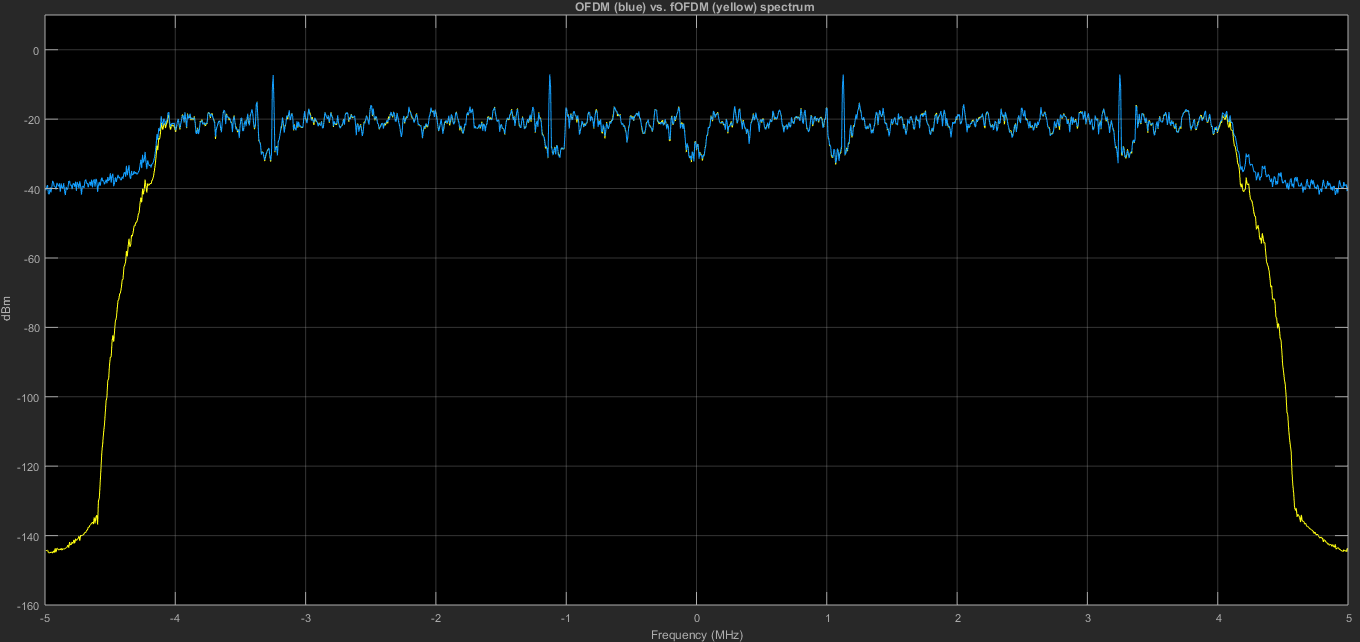
\includegraphics[width=8.5cm]{images/spectrum.png}
\caption{Magnitude spectrum for (blue) OFDM signal and (yellow) f-OFDM signal. Source: own.}
\label{fig:spectrum} 
\end{center}
\end{figure}

The results in amplitude are clearly seen. First the OFDM spectrum decays from the regular level to -40dBm in a step of 1 MHz, then the f-OFDM spectrum attenuates to a lvel of -140dBm in a frequency step even lower. Some of the guard bands in the f-OFDM signal was filtered, but since they do not hold any information this strategy will not harm the quality of reception. Anyway a big portion of the spectra was freed to use in adjacent communication channel, since the possibility of inter channel interference was reduced by the filtering.

Finally, since the time signal is a complex number (the conjugate symmetry property of IFFT was not ensured in the transmitter) it can be observed parsing into real and imaginary components. The plot in figure \ref{fig:time} shows the OFDM and fOFDM time signal. In the time domain the difference it is not clear, turning the spectral analysis a better tool to work with filter designs in the fOFDM context.

\begin{figure}[h]
\begin{center}
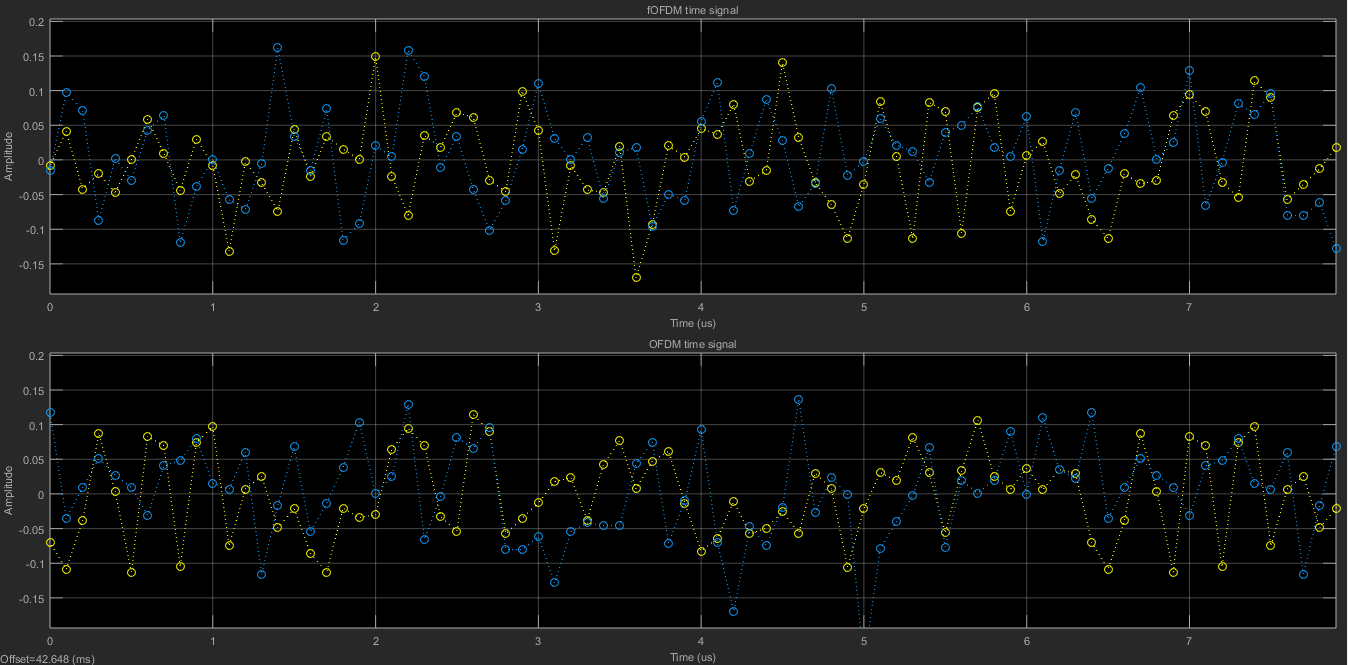
\includegraphics[width=8.5cm]{images/time.png}
\caption{fOFDM signal in time domain (top) and the original OFDM signal (bottom), and the yellow components represents the real part of the signal and the blue represents the imaginary part. Source: own.}
\label{fig:time} 
\end{center}
\end{figure}